\section*{写在前面}
本文主要记录吉林大学实变函数课程(曹阳)的笔记和课程总结.吉林大学实变函数主要包括以下的内容:1.集合论、2.测度论、3.可测函数、4.勒贝格(Lebesgue(下略)积分和勒贝格测度、5.\(L^2\)空间和\(L^n\)空间.本课程有期中考试.课程的主要难点在于对于测度理论的理解和对多种可测函数的了解.(复变函数惨剧不能在实变函数重演)
\section{前置知识}
在正式学习实变函数之前,我们需要了解一些前置知识,这些知识包括集合论以及它的附属内容.
\subsection{集合论}
在高中期间,就给出了集合的定义即:具有某种特定性质或同一关系的“事物”的总体,“事物“称为集合的元素.当两个集合相等时,我们一般认为是两个集合的元素完全相同
若一个集合A包含于另一个集合B,则代表集合A中的元素在集合B中都存在.我们称集合A为集合B的子集.若集合A不包含于集合B,则称集合A不是集合B的子集.我们称集合A为集合B的真子集.我们用符号\(\subset\)表示包含关系,用符号\(\subseteq\)表示包含关系或相等关系.
不含任何元素的集合称为虚无集或者空集,记为\(\emptyset\) 
\begin{Theorem}
    A=B的充要条件是:A\(\subset\)B且B\(\subset\)A    
\end{Theorem}
\begin{Theorem}
    如果\(A \subset B ,B \subset C\),则\(A \subset C\)
\end{Theorem}
\begin{Theorem}
    对于任意集合A,B,C,有如下公式成立:
    \begin{itemize}[itemsep=2pt,topsep=0pt,parsep=0pt]
        \item \(A \cup B = B \cup A , A \cap B = B \cap A\) \\
        \item \(A \cup (B \cup C) = (A \cup B) \cup C , A \cap (B \cap C) = (A \cap B) \cap C\) \\
        \item \(A \cup (B \cap C) = (A \cup B) \cap (A \cup C) , A \cap (B \cup C) = (A \cap B) \cup (A \cap C)\) \\
        \item \(A \cup \emptyset = A , A \cap \emptyset = \emptyset\) \\
        \item \(A \cup A^c = U , A \cap A^c = \emptyset\) \\
        \item \(A \cup U = U , A \cap U = A\) \\
        \item \(A \cup A =A , A \cap A = A\) \\
    \end{itemize}
\end{Theorem}
\begin{Theorem}
    \begin{itemize}[itemsep=2pt,topsep=0pt,parsep=0pt]
        \item \(A \cap B \subset A \subset A \cup B \) \\
        \item 若\(A_{\lambda} \subset B_{\lambda}\) 则\(\bigcup\limits_{\lambda \in \Lambda} A_{\lambda} \subset \bigcup\limits_{\lambda \in \Lambda} B_{\lambda}\) ,特别的是若\(A_{\lambda} \subset  C (\lambda \in \Lambda)\),则 \(\bigcup\limits_{\lambda \in \Lambda} A_{\lambda} \subset C\)\\
        \item 若\(A_{\lambda} \supset B_{\lambda} \) 则\(\bigcap\limits_{\lambda \in \Lambda} A_{\lambda} \supset \bigcap\limits_{\lambda \in \Lambda} B_{\lambda}\),特别的是若 \(B_{\lambda} \supset C (\lambda \in \Lambda)\) 则 \(\bigcap\limits_{\lambda \in \Lambda} B_{\lambda}\supset C \)\\ 
        \item \(\bigcup\limits_{\lambda \in \Lambda}(A_{\lambda} \cup B_{\lambda})=\bigl(\bigcup\limits_{\lambda \in \Lambda} A_{\lambda}\bigr) \bigcup \bigl(\bigcup\limits_{\lambda \in \Lambda} B_{\lambda}\bigr)\) \\
        \item \(A \bigcap \bigl(\bigcup\limits_{\lambda \in \Lambda} B_{\lambda}\bigr) = \bigcup\limits_{\lambda \in \Lambda} \bigl(A \cap B_{\lambda}\bigr)\)
    \end{itemize}
\end{Theorem}
\begin{Theorem}
    对于任意集合A,B,有如下公式成立:
    \begin{itemize}[itemsep=2pt,topsep=0pt,parsep=0pt]
        \item \(A \cup B = B \cup A , A \cap B = B \cap A\) \\
        \item \(A \cup (B \cup C) = (A \cup B) \cup C , A \cap (B \cap C) = (A \cap B) \cap C\) \\
        \item \(A \cup (B \cap C) = (A \cup B) \cap (A \cup C) , A \cap (B \cup C) = (A \cap B) \cup (A \cap C)\) \\
        \item \(A \cup \emptyset = A , A \cap \emptyset = \emptyset\) \\
        \item \(A \cup U = U , A \cap U = A\) \\
        \item \(A \cup A =A , A \cap A = A \)\\
    \end{itemize}
\end{Theorem}
\begin{Definition}
    对于两个不同集合A,B:我们定义如下运算:
    \[A-B := \left\{x ; x\in A \text{且} x \notin B\right\}\]
    我们称上述的运算为集合的差运算,有时候也称为集合的减法运算.
\end{Definition}
\begin{Theorem}
   \(A-B = A \cap B^c\)
\end{Theorem}
\begin{proof}
   \(\Rightarrow\)根据定义可知,对于\(x\in (A-B)\)来说:\(x \in A\)且\(x \in B^c\)从而可知\(x \in A \cap B^c\) \\ 
   \(\Leftarrow\) 反之依然 .
\end{proof}
\begin{Theorem}
    \begin{itemize}[itemsep=2pt,topsep=0pt,parsep=0pt]
        给定一个集合S,A是S的子集
        \item \(S^c = \emptyset ; \emptyset^c = \emptyset \) \\ 
        \item \(A \cup A^c = S ; A \cap A^c = \emptyset \)\\
        \item \((A^c)^c = A \)\\
        \item 若\(A \subset B \) ,则 \(A^c \supset B^c\)
    \end{itemize}
\end{Theorem}

\begin{Definition}
    对于一个给定的集合S,若 \(\mathscr{F}\)是S的一族子集,即\(\mathscr{F}\)是以S的一些子集为元素的一个集合,如果它满足如下条件: \\ 
    (1): \(\emptyset \in \mathscr{F}\) \\ 
    (2): 若\(A \in \mathscr{F}\),则\(A^c \in \mathscr{F}\) \\ 
    (3): 若\(A_1,A_2,\dots,A_n \in \mathscr{F}\),则\(\bigcup\limits_{i=1}^{n} A_i \in \mathscr{F}\) \\
    我们称这样的\(\mathscr{F}\)为S的一个\(\sigma\)-代数.
\end{Definition}
\begin{Theorem}
    如果\(\mathscr{A}\) 是由S的子集构成的一个非空集合,则存在唯一一个S的子集的\(\sigma\)-域\(\mathscr{F} (\mathscr{A})\),是\(\mathscr{A} \subset \mathscr{F}(\mathscr{A})\)并且对于S的子集的的任何\(\sigma\)-域\(\mathscr{F}\),只要\(\mathscr{F} \subset \mathscr{A}\) , 就有\(\mathscr{F} \subset \mathscr{F}(\mathscr{F})\),这也就是说在S的子集的包含\(\mathscr{A}\)的\(\sigma\)-域 中有一个最小的\(\mathscr{F}(\mathscr{A})\).这个\(\sigma\)-域\(\mathscr{F}(\mathscr{A})\)称为由\(\mathscr{A}\)产生的\(\sigma\)-域.
\end{Theorem}
对于一串给定的集合\(A_1,A_2 ,\dots , A_n , \dots  \) 我们定义 \[x ; 有无穷多个n , 使得 x \in A_n\]
为这串集合的上极限,记为\(\limsup_{n} A_n \)或者\(\overline{\lim_{n}}A_n\);
定义 \[ x ; 有有限多个n , 使得x \notin A_n\]
为这串集合的下极限,记为  \(\liminf_{n}A_n\) 或者\(\widetilde{\lim_{n}}A_n\).
如果集合列的上,下极限均存在且相等,那么它的上下极限统称为极限,记为\(\lim_{n}A_n\).
\begin{Theorem}
    对于一串给定的集合\(A_1,A_2 ,\dots , A_n , \dots  \) 我们有如下结论:
    \begin{itemize}[itemsep=2pt,topsep=0pt,parsep=0pt]
        \item \(\limsup_{n} A_n = \bigcap\limits_{n=1}^{\infty} \bigcup\limits_{k=n}^{\infty} A_k\) \\
        \item \(\liminf_{n} A_n = \bigcup\limits_{n=1}^{\infty} \bigcap\limits_{k=n}^{\infty} A_k\) \\
    \end{itemize}
\end{Theorem}
\begin{Theorem}
    给定一个集合列\(A_1 , A_2 \dots A_n \dots \) ,我们有如下结论: \\ 
    (1):如果集合列是(单调)递增的即\(A_n \subset A_{n+1}\) 则 \(\lim_{n}A_n = \bigcup\limits_{i=1}^{\infty} A_n\) \\
    (2):如果集合列是(单调)递减的即\(A_n \supset A_{n+1}\) 则 \(\lim_{n}A_n = \bigcap\limits_{i=1}^{\infty} A_n\) \\
\end{Theorem}
\section{第一周}
\subsection{素扑集合论}
在数学分析中,我们初步了解了集合的定义、定理、应用.这些似乎都是正确的.但1903年英国数学家罗素提出了罗素悖论即讨论如下问题:一个集合的集合是否是集合.为了使得上述命题具有良定义,罗素并未直接使用集合的集合而是运用了另一种等价命题.
\begin{Example}[罗素悖论]
    假定一个集合\(\mathrm{W}  \notin \mathrm{W}\),那么不妨取如下集合
    \[\widetilde{W} =  \left\{\mathrm{V} \subset \mathrm{W}|  \mathrm{V} \notin \mathrm{V} \right\}\]
    上述集合揭示了一个矛盾: 
                \[\mathrm{W} \in \mathrm{W}\]
\end{Example}
罗素悖论让数学家猛然发现原有集合论出现了危机,但是我们不对上述问题进一步讨论,留作线上作业(自行阅读文献\url{https://mathshistory.st-andrews.ac.uk/HistTopics/Beginnings_of_set_theory/}).
\\
在素扑集合论中,Cantor首次引用了势(又称基数)的概念.
\begin{Definition}
    对于集合A来说,集合A的基数就是集合A中所有元素的个数,记作\(\overline{\overline{A}}\) 
\end{Definition}
通常情况下,对于两个集合A,B: 如果A到B的映射是单射,那么称A的基数小于B的基数.如果A到B的映射既单又满,那么称A和B是等势的(一一对应).
紧接着,Cantor通过观察发现\([0,1]\)和自然数集\(\mathbf{N}\)之间基数不相等从而引发了对于无穷大是否是“真”无穷大的讨论.下面系统地给出\([0,1]\)和自然数集\(\mathbf{N}\)之间基数关系
\begin{Theorem}
\([0,1]\)的基数大于自然数集\(\mathbf{N}\) 即:
   \[ \overline{\overline{([0,1])}} \succ \overline{\overline{\mathbf{N}}}\]
\end{Theorem}
接下来我们使用两种方法进行证明:
\begin{proof}[三分法]
    首先可知自然数集是可数集\footnote{此性质见数学分析(陈纪修)},那么不妨取自然数集全体为\(x_0 , x_1 ,x_2 \dots x_n \dots \).考虑\([0,1]\) :使用三分法(如图\ref{fig:enter-label_1})即\[[0,1] = [0 \frac{1}{3}] \cup [\frac{1}{3}, \frac{2}{3}] \cup [\frac{2}{3}, 1 ] \] 假如我们只选取\([\frac{2}{3} ,1 ] \),那么自然数集中元素一定有不在\([\frac{2}{3}, 1 ]\)中的,不断重复,一定能得到如下结论:存在一个集合A,不包含任何自然数集中的元素.但是有根据闭区间套定理或者Cantor定理我们可知集合A非空.得证.
\end{proof}
虽然上面的证明方法很巧妙但是没有得到当时主流数学家的认可. 
\begin{figure}[h]
    \centering
    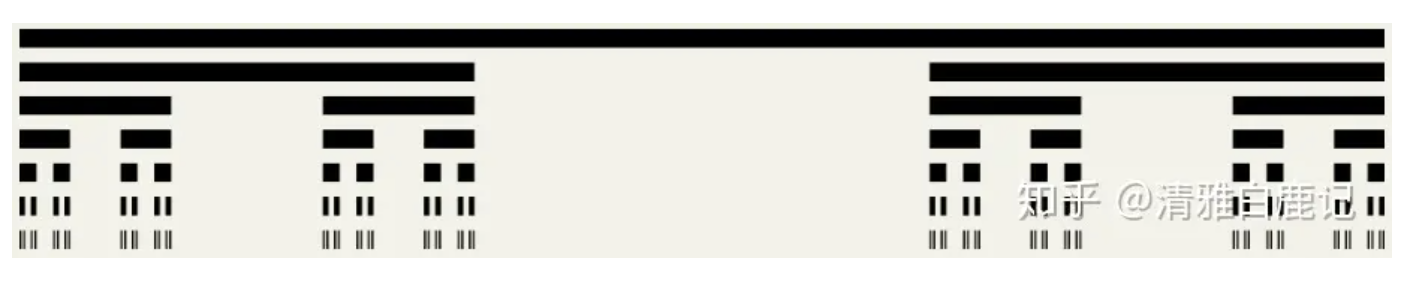
\includegraphics[width=0.5\linewidth]{figures/image_1.png}
    \caption{Cantor三分集}
    \label{fig:enter-label_1}
\end{figure}
下面我们使用对角线法进行证明
\begin{proof}[对角线法]
    首先我们可知\([0,1]\)中的元素均为如下形式\(0.x_0x_1x_2\dots\),其次通过数学分析中的操作可以将自然数集按照大小排列为矩阵形式即
\(   \begin{pmatrix}  
  1& \cdots & \cdots \\  
  n & \ddots & \vdots \\  
  \vdots & \cdots & \cdots  
\end{pmatrix} \) 
我们取上面矩阵的所有对角线元素来组成\([0,1]\)中的元素.不断重复以上操作,得证
\end{proof}
\subsection{无穷大}
对于无穷大来说:我们需要牢记以下性质:\\
\begin{itemize}
    \item 自然数集的基数和\([0,1]\)的基数不同,换而言之它们是不同的无穷大 \\
    \item 有无穷多个不同的无穷大 \\
    \item 没有最大的无穷大
\end{itemize}
\begin{Proposition}[连续统假设]
    不存在这样的集合,它的基数位于自然数集的基数和\([0,1]\)的基数之间.
\end{Proposition}
需要说明的是连续统假设在现有的ZFC证明体系中无法被证明,尽量不要使用,使用需预先声明
\subsection{Bernstein定理}
在素扑集合论中,我们要证明两个集合是等势的,要构造出这两个集合之间的双射,但是这步往往是困难重重.这时候Bernstein定理就起了很大的作用.
\begin{Theorem}[Bernstein]
    对于两个集合A,B: 若\(\overline{\overline{A}} \succ \overline{\overline{B}}\)且 \(\overline{\overline{B}} \succ \overline{\overline{A}}\)那么\(\overline{\overline{A}} = \overline{\overline{B}}\)
\end{Theorem}
\begin{proof}[Bernstein]
    考虑集合A,B之间的映射关系,取\(\varphi\)为A到B的单射,\(\gamma\)为B到A的单射.那么存在B中子集\(B_0\),使得\(\varphi\)是A到\(B_0\)的一一对应.同样的存在A中子集\(A_0\),使得\(\gamma\)是B到\(A_0\)的一一对应(如图\ref{fig:enter-label_2}).之后,我们对剩余部分进行二分法处理从而有如下式:
    \begin{align*}
        C &= A - A_0 - \bigcup\limits_{k=1}^{\infty} A_k \\
        &= \gamma(B) -\gamma(B-B_0) - \gamma(\bigcup\limits_{k=1}^{\infty} B_k) \\
        &=\gamma(B_0 -\bigcup\limits_{k=1}^{\infty} B_k)
    \end{align*}
    因此我们能够得到上述定理
\end{proof}
  \begin{figure}[h]
    \centering
    \includegraphics[width=0.25\linewidth]{PNG图像-747D08326374-1.png}
    \caption{}
    \label{fig:enter-label_2}
\end{figure}
或许有的人认为Bernstein定理是显然的,但是实际上证明十分困难.因为题目只给了两个条件:两个单射.Bernstein做法巧妙地避免的这种简陋的条件.运用迭代和图像的思想来证明.
\subsection{连续统基数(势)}
根据连续统假设,我们把\([0,1]\)的基数称为连续统基数,记为\(\aleph_0\)(为了书写方便,我们在实际使用当中常记为c)
\begin{Example}
    一些常见的基数为c的集合: 
    \begin{itemize}
        \item 实数集R \\
        \item 任何一个非空开区间 \\
        \item 一些基数小于等于c的集合,若他们当中有任意一个集合的基数为c,那么他们的并集 \\
        \item n维欧氏空间 \(R^n\)
    \end{itemize}
\end{Example}
\subsection{可数集合}
首先,先明晰一个概念:可数集合就是可列集合.为什么这么说呢:
\\ 
首先,可数集合的定义是:凡是能够和全体正整数组成的集合\(\mathcal{Z}_{+}\)对等的集合都称为可数集合.再回顾一下可列集合的定义:若一个集合能够和有理数集\(\mathcal{Q}\)对等,那么称这个集合为可列集合.那么我们不难发现:有理数集\(\mathcal{Q}\)和全体正整数组成的集合\(\mathcal{Z}_{+}\)是对等的,因此可数集合和可列集合是等价的.
因此,给出一个兼顾可数集合和可列集合的定义:
\begin{Definition}
    如果一个集合能够和全体正整数组成的集合\(\mathcal{Z}_{+}\)对等,那么称这个集合为可数集合.我们把这个集合的基数称为可数基数,记为\(\aleph_0\)或者c.
\end{Definition}
需要指出的是可数基数是\(\aleph_0\)事实上是不妥的,因为连续统假设并没有被证明.但是在实际使用中,我们常常把可数基数称为\(\aleph_0\).
下面给出一些定理:
\begin{Theorem}给定一个可列集合列\(A_i\): \\ 
    (1): 任何一个无穷集合都有可数子集 \\ 
    (2): 可数集合的自己如果不是有限集合,则一定还是可数集合 \\ 
    (3): 若A可数,B有限,则\(A \cup B\)可数 \\ 
    (4): 若A,B都是可数集合,则\(A \cup B\) 可数 \\ 
    (5): 如果\(A_i (i=1,2,3,\dots )\)的每一个都是可数集合,则\(\bigcup\limits_{i=1}^{\infty} A_i\)也是可数集合. \\ 
    (6): 全体有理数构成一个可数集合.  \\ 
    (7): 如果A是一无穷集合,B是一可数集合,则\(A\cup B \sim A\)
\end{Theorem}
\begin{proof}
    (1): 给定一个无穷集合A,从A中取得一个元素记为\(e_1\),那么同样的,从\(A - \left\{e_1\right\} \)我们取得第二个元素\(e_2\),不断重复以上操作,得到A的一个无穷可数子集 \[e_1, e_2,e_3, \dots e_n \dots \]
    (2):由(1)易知,证明略 . \\ 
    (3): 若A可数,那么它的元素可以按照一定次序排列即\[a_1,a_2,\dots , a_n \dots\]又因为B是有限集合,那么\(A \cup B\)中的元素可以按照如下次序排列
    \[a_1,b_1,a_2,b_2,\dots ,a_n,b_n \dots\]
    (4):若A,B都是可数集合,那么它们的元素可以按照一定次序排列即\(a_1,a_2,\dots , a_n \dots\)和\(b_1,b_2,\dots , b_n \dots\)那么\(A \cup B\)中的元素可以按照如下次序排列:\[a_1,b_1,\dots , a_n,b_n \dots \]
    (5):如果\(A_i (i=1,2,\dots)\)每一个都是可数集合,作如下构造: \\ 
    记\(A^{*}_1 = A_1  , A^{*}_i = A_i - \bigl(\bigcup\limits_{t=1}^{i-1} A_t\bigr)\)
    所以我们能够得到如下事实: \\ 
   \(A^{*}_i\)都是可数的,那么可以排列为如下形式 \[a_{i1},a_{i2},\dots,a_{in},\dots\]
   因此对于\[\bigcup\limits_{i=1}^{\infty} A^{*}_i = \left\{a_{ij} | i= 1, 2 \dots ;j = 1,2 ,dots \right\}\]
   并且令\(a_{ij}\)为整数\(2^i3^j\),由于正整数分解定理,可知当\(i_1\neq i_2, j_1 \neq j_2\) 时有\(2^{i_1}3^{j_1} \neq 2^{i_2}3^{j_2}\),所以:\[\bigcup\limits_{i=1}^{\infty} A_i=\bigcup\limits_{i=1}^{\infty} A^{*}_i \text{是可数集合} \] 
   \\ 
   (6): 考虑有理数的笛卡尔积\(\mathcal{Z} \times \mathcal{Z}\),我们有:\[f:\mathcal{Z} \times \mathcal{Z} \rightarrow Q \quad f(p,q)=\frac{p}{q} \]根据上述可知,有理数集是可数集合. \\ 
   (7): 
\end{proof}
\begin{Theorem}
    有限多个可数集的乘积是可数集
\end{Theorem}
\begin{proof}
    设\(A_1,A_2,\dots,A_n\)为可数集,则\[\prod_{i=1}^{n} A_i = \left\{x_{1j_1}, x_{2j_2} ,\dots,x_{n,j_n} \right\} \quad x_{ij_i} \in A+\i\]
    并且\begin{align*}
        f(\alpha) = \prod_{i=1}^{n}p_{i}^{j_i} \quad p_i\text{为不同的质数} \quad \alpha \in prod_{i=1}^{n} A_i
    \end{align*}
    则\(f(\alpha)\)为一一对应,于是有限多个可数集的乘积是可数集
\end{proof}
